\frame
{
\frametitle{Selección Clonal}
\framesubtitle{Algoritmo}

\begin{itemize}
    \item Generar un conjunto (P) de \blue{soluciones candidatas},
		compuesto de \green{células de memoria} (M) añadidas a la
		\green{población restante} (Pr), teniendo entonces $P = Pr + M$
    \item Determinar los $n$ \blue{mejores individuos} (Pn) de la población (P),
		basado en una medida de \red{afinidad}.
    \item Clonar (reproducir) estos $n$ mejores individuos de la población,
		dando origen a una \blue{población temporal de clones} (C).
\end{itemize}
}

\frame
{
\frametitle{Selección Clonal}
\framesubtitle{Algoritmo}

\begin{itemize}
    \item Someter la población de clones a un esquema de \blue{hiper-mutación}
		Una población de \green{anticuerpos maduros} es generada (C*).
    \item Seleccionar nuevamente los \red{mejores} individuos de (C*)
		para componer el \green{conjunto de memoria}.
    \item Reemplazar los $d$ anticuerpos con \blue{menor afinidad} de la población,
		manteniendo la \red{diversidad}.
\end{itemize}

}

\frame
{
\frametitle{Selección Clonal}
\framesubtitle{Algoritmo}
\begin{center}
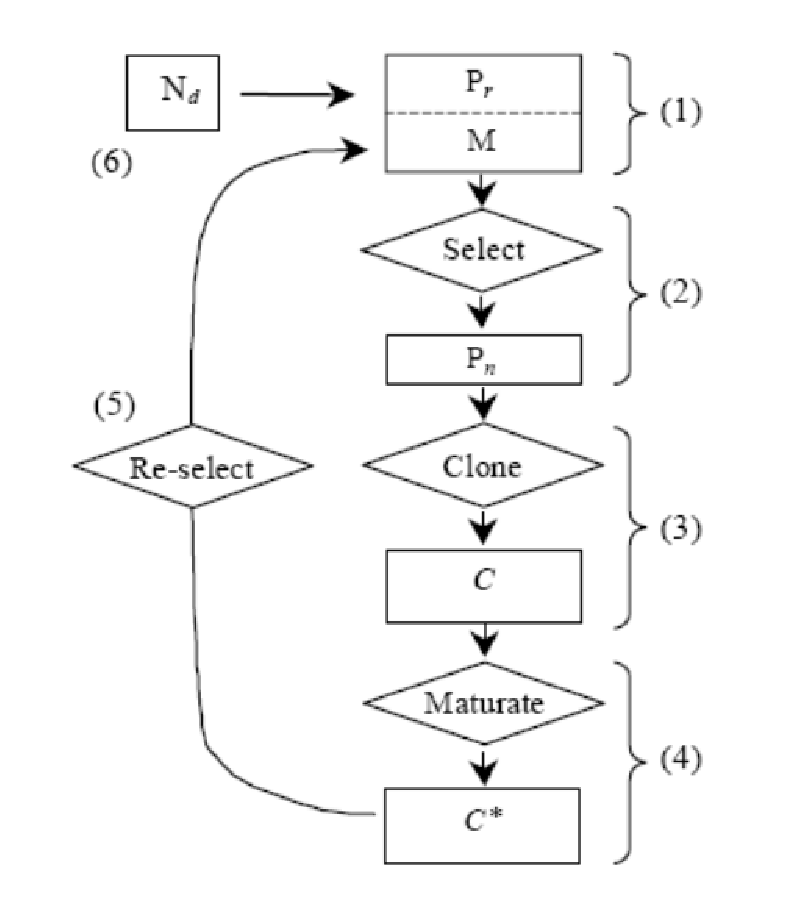
\includegraphics[width=0.5\textwidth]{../doc/img/algoritmo}
\end{center}
}
